\apendice{Especificación de Requisitos}

\section{Introducción}
En este apartado se enumerarán y desarrollarán los objetivos y requisitos que debe tener la aplicación según han sido marcados al comienzo del proyecto. Además de estos, se han añadido algunos a lo largo del desarrollo.

\section{Objetivos generales}
Este proyecto tiene como objetivo los siguientes puntos:
\begin{itemize}
\tightlist
    \item Crear una aplicación que permita realizar análisis de sentimiento a textos extraídos de las redes sociales twitter e instagram.
    \item Almacenar dicha información en una base de datos para que sea fácilmente accesible.
    \item Mostrar dicha información en gráficos y tablas para poder analizar los datos de análisis.
    \item Calcular series temporales para la predicción de valores futuros.
    \item Crear una wiki para el manual de usuario.
\end{itemize}
\newpage
\section{Catálogo de requisitos}
En este apartado se definirán los requisitos funcionales y no funcionales del proyecto.
\subsection{Requisitos funcionales}
\begin{itemize}
\tightlist
    \item \textbf{RF1-Registro de usuarios:} La aplicación debe permitir a un usuario crearse una cuenta y que sus datos sean almacenados en la base de datos.
    \item \textbf{RF2-Login de usuarios:} La aplicación debe ser capaz de dadas las credenciales de un usuario permitirle acceder a las funcionalidades.
    \item \textbf{RF3-Información de la aplicación:} El usuario debe poder obtener información de cómo funciona la aplicación.
    \item \textbf{RF4-Analizar textos:} La aplicación debe ser capaz de analizar textos.
        \begin{itemize}
        \tightlist
            \item \textbf{RF4.1-Acceder a las APIs:} La aplicación debe acceder a las APIs de twitter e instagram.
            \item \textbf{RF4.2-Extraer textos:} La aplicación debe ser capaz de extraer los textos de las APIs.
            \begin{itemize}
            \tightlist
                \item \textbf{RF4.2.1-Extraer textos de twitter:} La aplicación debe extraer tweets de la API dado un hashtag, un usuario o una palabra.
                \item \textbf{RF4.2.2-Extraer textos de instagram:} La aplicación debe extraer los comentarios de las publicaciones de un perfil dado un usuario.
            \end{itemize}
            \item \textbf{RF4.3-Puntuar los textos:} La aplicación debe realizar el análisis del texto obtenido y devolver un valor decimal entre -1 y 1.
            \item \textbf{RF4.4-Almacenar resultados:} La aplicación debe almacenar las puntuaciones junto con el texto analizado, fecha en la que se escribió y el identificador.
        \end{itemize}
        \item \textbf{RF5-Realizar estadísticas:} La aplicación debe calcular la media, moda, mediana, varianza y desviación típica de los valores almacenados de cada identificador.
        \item\textbf{RF6-Buscar resultados por identificador:} El usuario debe poder buscar los resultados de un identificador con unas fechas seleccionadas.
        \begin{itemize}
        \tightlist
            \item \textbf{RF6.1-Buscar por hashtag:} El usuario debe poder introducir un hashtag y ver los resultados del análisis en gráficos.
            \item \textbf{RF6.2-Buscar por usuario de twitter:} El usuario debe poder buscar un usuario de twitter y visualizar el análisis de los textos en los que ha sido mencionado.
            \item\textbf{RF6.3-Buscar por palabra:} El usuario debe poder buscar una palabra para ver los resultados del análisis de los textos en los que está esa palabra.
            \item\textbf{RF6.4-Buscar por usuario de instagram:} El usuario debe poder buscar un usuario de instagram para ver los análisis de los comentarios de las publicaciones del perfil.
        \end{itemize}
        \item \textbf{RF7-Mostrar gráficos:} La aplicación debe mostrar los resultados de análisis en gráficas y tablas.
        \begin{itemize}
        \tightlist
            \item \textbf{RF7.1-Gráfico de resultados del análisis:} Debe mostrar un gráfico de barras de todos los datos del análisis de un identificador en las fechas indicadas.
            \item\textbf{RF7.2-Tabla de resultados del análisis:} Debe mostrar todos los datos del análisis de un identificador en las fechas indicadas junto al texto que ha sido analizado.
            \item\textbf{RF7.3-Gráfico de media por días:} Debe mostrar un gráfico lineal de la media de los resultados por días.
            \item\textbf{RF7.4-Gráfico de intervalos:} Debe mostrar un gráfico de barras con los datos agrupados por intervalos.
            \begin{itemize}
                \item\textbf{RF7.4.1-Gráfico de intervalos fijos:} Debe mostrar los datos agrupados en intervalos de 0.1 entre el 0 y 1.
                \item\textbf{RF7.4.2-Gráfico de intervalos dinámicos:} Debe mostrar los datos agrupados en intervalos de 0.1 entre el menor valor y el mayor.
            \end{itemize}
            \item\textbf{RF7.5-Gráfico Sentinel trends:} Debe mostrar en un gráfico circular el número de resultados que pertenecen a ese identificador en las fechas seleccionadas entre el total de resultados de la opción escogida.
        \end{itemize}
        \item\textbf{RF8-Calcular series temporales:} La aplicación calculará series temporales a partir de los resultados del análisis y las elecciones del usuario. 
        \item\textbf{RF9-Configurar idioma:} El usuario debe poder cambiar el idioma de la aplicación.
\end{itemize}

\newpage
\subsection{Requisitos no funcionales}
\begin{itemize}
\tightlist
    \item \textbf{RNF1-Usabilidad:} La aplicación debe ser \textit{user friendly} para que la experiencia del usuario sea lo más positiva posible. Además debe poder adaptarse a diferentes formatos de pantalla, es decir que sea \textit{responsive}.
    \item \textbf{RNF2-Eficiencia:} El almacenamiento de resultados en la base de datos y la respuesta de la aplicación al navegar entre ventanas, sobre todo, al mostrar los gráficos debe ser lo más rápido posible.
    \item \textbf{RNF3-Disponibilidad:} La aplicación debe estar disponible durante el mayor tiempo posible y en la mayoría de lugares.
    \item \textbf{RNF4-Escalabilidad:} La aplicación debe estar preparada para soportar nuevos desarrollos que generen mayor cantidad de trabajo.
    \item \textbf{RNF5-Confiabilidad:} La aplicación cumplirá la función para la que se ha creado.
    \item \textbf{RNF6-Mantenibilidad:} La aplicación debe permitir cambios y correcciones de forma eficaz. 
    \item \textbf{RNF7-Internacionalización:} La aplicación debe soportar varios idiomas.
    
\end{itemize}
\clearpage

\section{Especificación de requisitos}

\subsection{Casos de uso}

\begin{table}[ht!]
    \centering
    \resizebox{15cm}{!} {
    \begin{tabular}{|l|l|}
    \hline
         \textbf{CU-01}     &  \textbf{Registro de usuarios} \\ \hline
         \textbf{Requisitos relacionados}       & RF1 \\ \hline
         \textbf{Descripción}    & Permite al usuario crearse una cuenta. \\ \hline   
         \textbf{Precondiciones}      & La base de datos debe estar disponible. \\ \hline
         \textbf{Acciones}      &  \parbox[p][0.2\textwidth][c]{10cm}{
            \begin{enumerate}\tightlist
                 \item El usuario accede a la opción Crear cuenta.
                 \item El usuario introduce su nombre, apellidos, identificador de usuario y contraseña.
                 \item Pulsa el botón de registrarse.
            \end{enumerate}} \\ \hline
         \textbf{Postcondiciones}       & El identificador de usuario no debe existir en la base de datos. \\ \hline
         \textbf{Excepciones}       & \parbox[p][0.1\textwidth][c]{10cm}{
         \begin{enumerate}\tightlist
             \item El identificador de usuario ya existe (mensaje).
             \item Carácter incorrecto (mensaje).
         \end{enumerate}} \\ \hline
         \textbf{Importancia}   &Alta. \\
         \hline
    \end{tabular}}
    \caption{CU01 - Registro de usuarios}
    \label{tab:my_label}
\end{table}

\begin{table}[ht!]
    \centering
    \resizebox{15cm}{!} {
    \begin{tabular}{|l|l|}
    \hline
         \textbf{CU-02}     &  \textbf{Login de usuarios} \\ \hline
         \textbf{Requisitos relacionados}       & RF2 \\ \hline
         \textbf{Descripción}    & Permite al usuario acceder a la aplicación. \\ \hline   
         \textbf{Precondiciones}      & El usuario debe estar registrado. \\ \hline
         \textbf{Acciones}      &  \parbox[p][0.2\textwidth][c]{10cm}{
            \begin{enumerate}\tightlist
                 \item El usuario accede a la opción Login.
                 \item El usuario introduce su identificador de usuario y contraseña.
                 \item Pulsa el botón de acceder.
            \end{enumerate}} \\ \hline
         \textbf{Postcondiciones}       & El identificador de usuario y la contraseña deben existir en la base de datos. \\ \hline
         \textbf{Excepciones}       & El identificador de usuario o contraseña no son correctos (mensaje). \\ \hline
         \textbf{Importancia}   &Alta. \\
         \hline
    \end{tabular}}
    \caption{CU02 - Login de usuarios}
    \label{tab:my_label}
\end{table}

\begin{table}[ht!]
    \centering
    \resizebox{15cm}{!} {
    \begin{tabular}{|l|l|}
    \hline
         \textbf{CU-03}     &  \textbf{Información de la aplicación} \\ \hline
         \textbf{Requisitos relacionados}       & RF3 \\ \hline
         \textbf{Descripción}    & Permite al usuario obtener información sobre la aplicación. \\ \hline   
         \textbf{Precondiciones}      & - \\ \hline
         \textbf{Acciones}      & El usuario accede a la opción información. \\ \hline
         \textbf{Postcondiciones}       & - \\ \hline
         \textbf{Excepciones}       & - \\ \hline
         \textbf{Importancia}   &Baja. \\
         \hline
    \end{tabular}}
    \caption{CU03 - Información de la aplicación}
    \label{tab:my_label}
\end{table}

\begin{table}[ht!]
    \centering
    \resizebox{15cm}{!} {
    \begin{tabular}{|l|l|}
    \hline
         \textbf{CU-04}     &  \textbf{Acceder a las APIs} \\ \hline
         \textbf{Requisitos relacionados}       & RF4.1 \\ \hline
         \textbf{Descripción}    & Permite acceder a los datos de las APIs de twitter e instagram. \\ \hline   
         \textbf{Precondiciones}      &\parbox[p][0.1\textwidth][c]{10cm}{
            \begin{enumerate}\tightlist
                \item Tener cuenta developer de twitter.
                \item Tener cuenta de instagram.
            \end{enumerate}}\\ \hline
         \textbf{Acciones}      & Se realiza la conexión con cada API a través de las cuentas personales.\\ \hline
         \textbf{Postcondiciones}       & - \\ \hline
         \textbf{Excepciones}       &- \\ \hline
         \textbf{Importancia}   & Alta.\\
         \hline
    \end{tabular}}
    \caption{CU04 - Acceder a las APIs}
    \label{tab:my_label}
\end{table}

\begin{table}[ht!]
    \centering
    \resizebox{15cm}{!} {
    \begin{tabular}{|l|l|}
    \hline
         \textbf{CU-05}     &  \textbf{Extraer textos} \\ \hline
         \textbf{Requisitos relacionados}       & RF4.2, RF4.2.1, RF4.2.2 \\ \hline
         \textbf{Descripción}    & Permite extraer textos de twitter e instagram. \\ \hline   
         \textbf{Precondiciones}      & Haber accedido a las APIs.\\ \hline
         \textbf{Acciones}      & Se extraen los textos filtrando por identificador.\\ \hline
         \textbf{Postcondiciones}       & - \\ \hline
         \textbf{Excepciones}       &- \\ \hline
         \textbf{Importancia}   & Alta.\\
         \hline
    \end{tabular}}
    \caption{CU05 - Extraer textos}
    \label{tab:my_label}
\end{table}

\begin{table}[ht!]
    \centering
    \resizebox{15cm}{!} {
    \begin{tabular}{|l|l|}
    \hline
         \textbf{CU-06}     &  \textbf{Extraer textos de twitter} \\ \hline
         \textbf{Requisitos relacionados}       & RF4.2, RF4.2.1 \\ \hline
         \textbf{Descripción}    & Permite extraer textos de twitter. \\ \hline   
         \textbf{Precondiciones}      & Haber accedido a la API de twitter.\\ \hline
         \textbf{Acciones}      &
         \parbox[p][0.2\textwidth][c]{10cm}{
            \begin{enumerate}\tightlist
            \item Se proporciona un identificador que puede ser un hashtag, un usuario de twitter o una palabra.
            \item Se extraen los tweets referentes al identificador dado.
            \end{enumerate}}\\ \hline
         \textbf{Postcondiciones}       & - \\ \hline
         \textbf{Excepciones}       &- \\ \hline
         \textbf{Importancia}   & Alta.\\
         \hline
    \end{tabular}}
    \caption{CU06 - Extraer textos de twitter}
    \label{tab:my_label}
\end{table}

\begin{table}[ht!]
    \centering
    \resizebox{15cm}{!} {
    \begin{tabular}{|l|l|}
    \hline
         \textbf{CU-07}     &  \textbf{Extraer textos de instagram} \\ \hline
         \textbf{Requisitos relacionados}       & RF4.2, RF4.2.2 \\ \hline
         \textbf{Descripción}    & Permite extraer textos de instagram. \\ \hline   
         \textbf{Precondiciones}      & Haber accedido a la API de instagram.\\ \hline
         \textbf{Acciones}      & \parbox[p][0.2\textwidth][c]{10cm}{
            \begin{enumerate}\tightlist
            \item Se proporciona un identificador que será un usuario de instagram.
            \item Se extraen los comentarios de todos los post de ese perfil.
            \end{enumerate}}\\ \hline
         \textbf{Postcondiciones}       & - \\ \hline
         \textbf{Excepciones}       &- \\ \hline
         \textbf{Importancia}   & Alta.\\
         \hline
    \end{tabular}}
    \caption{CU07 - Extraer textos de instagram}
    \label{tab:my_label}
\end{table}

\begin{table}[ht!]
    \centering
    \resizebox{15cm}{!} {
    \begin{tabular}{|l|l|}
    \hline
         \textbf{CU-08}     &  \textbf{Puntuar los textos} \\ \hline
         \textbf{Requisitos relacionados}       & RF4.3 \\ \hline
         \textbf{Descripción}    & Permite puntuar los textos. \\ \hline   
         \textbf{Precondiciones}      & Haber recogido textos de twitter o instagram.\\ \hline
         \textbf{Acciones}      & Se proporciona un texto al analizador de sentimiento. \\ \hline
         \textbf{Postcondiciones}       & - \\ \hline
         \textbf{Excepciones}       &- \\ \hline
         \textbf{Importancia}   & Alta.\\
         \hline
    \end{tabular}}
    \caption{CU08 - Puntuar los textos}
    \label{tab:my_label}
\end{table}


\begin{table}[ht!]
    \centering
    \resizebox{15cm}{!} {
    \begin{tabular}{|l|l|}
    \hline
         \textbf{CU-09}     &  \textbf{Almacenar los resultados} \\ \hline
         \textbf{Requisitos relacionados}       & RF4, RF4.4 \\ \hline
         \textbf{Descripción}    & Almacena en base de datos los resultados. \\ \hline   
         \textbf{Precondiciones}      & Haber obtenido resultados de analizar los textos.\\ \hline
         \textbf{Acciones}      & Se almacena el resultado del análisis junto al texto, el identificador \\ &y la fecha de creación de dicho texto. \\ \hline
         \textbf{Postcondiciones}       & - \\ \hline
         \textbf{Excepciones}       &- \\ \hline
         \textbf{Importancia}   & Alta.\\
         \hline
    \end{tabular}}
    \caption{CU09 - Almacenar los resultados}
    \label{tab:my_label}
\end{table}


\begin{table}[ht!]
    \centering
    \resizebox{15cm}{!} {
    \begin{tabular}{|l|l|}
    \hline
         \textbf{CU-10}     &  \textbf{Realizar estadísticas} \\ \hline
         \textbf{Requisitos relacionados}       & RF5 \\ \hline
         \textbf{Descripción}    & Realiza estadísticas de los resultados del análisis. \\ \hline   
         \textbf{Precondiciones}      & Almacenar los datos recogidos con su identificador.\\ \hline
         \textbf{Acciones}      & \parbox[p][0.3\textwidth][c]{10cm}{
            \begin{enumerate}\tightlist
            \item Recoge todos los datos referentes a un identificador.
            \item Calcula la media, moda, mediana, varianza y desviación típica.
            \item Almacena en la base de datos los resultados junto al identificador.
            \item Si el identificador ya había sido introducido se actualizan los datos.
            \end{enumerate}}\\ \hline
         \textbf{Postcondiciones}       & - \\ \hline
         \textbf{Excepciones}       &- \\ \hline
         \textbf{Importancia}   & Media.\\
         \hline
    \end{tabular}}
    \caption{CU10 - Realizar estadísticas}
    \label{tab:my_label}
\end{table}


\begin{table}[ht!]
    \centering
    \resizebox{15cm}{!} {
    \begin{tabular}{|l|l|}
    \hline
         \textbf{CU-11}     &  \textbf{Buscar resultados por identificador} \\ \hline
         \textbf{Requisitos relacionados}       & RF6, RF6.1, RF6.2, RF6.3, RF6.4 \\ \hline
         \textbf{Descripción}    & Permite buscar los resultados del análisis por su identificador. \\ \hline   
         \textbf{Precondiciones}      & Haber accedido a la aplicación.\\ \hline
         \textbf{Acciones}      & \parbox[p][0.2\textwidth][c]{10cm}{
            \begin{enumerate}\tightlist
            \item Se escoge si se quiere buscar en twitter o en instagram.
            \item Se proporciona un identificador.
            \item Se pulsa el botón de analizar.
            \end{enumerate}}\\ \hline
         \textbf{Postcondiciones}       & - \\ \hline
         \textbf{Excepciones}       &Carácter introducido no válido (mensaje). \\ \hline
         \textbf{Importancia}   & Alta.\\
         \hline
    \end{tabular}}
    \caption{CU11 - Buscar resultados por identificador}
    \label{tab:my_label}
\end{table}

\begin{table}[ht!]
    \centering
    \resizebox{15cm}{!} {
    \begin{tabular}{|l|l|}
    \hline
         \textbf{CU-12}     &  \textbf{Buscar por hashtag} \\ \hline
         \textbf{Requisitos relacionados}       & RF6, RF6.1 \\ \hline
         \textbf{Descripción}    & Permite buscar los resultados de hashtags. \\ \hline   
         \textbf{Precondiciones}      & Haber escogido analizar en twitter.\\ \hline
         \textbf{Acciones}      & \parbox[p][0.2\textwidth][c]{10cm}{
            \begin{enumerate}\tightlist
            \item Se introduce un identificador que empiece por \textit{\#}.
            \item Se selecciona una fecha si se quiere.
            \item Se pulsa el botón de analizar.
            \end{enumerate}}\\ \hline
         \textbf{Postcondiciones}       & - \\ \hline
         \textbf{Excepciones}       &- \\ \hline
         \textbf{Importancia}   & Alta.\\
         \hline
    \end{tabular}}
    \caption{CU12 - Buscar por hashtag}
    \label{tab:my_label}
\end{table}

\begin{table}[ht!]
    \centering
    \resizebox{15cm}{!} {
    \begin{tabular}{|l|l|}
    \hline
         \textbf{CU-13}     &  \textbf{Buscar por usuario de twitter} \\ \hline
         \textbf{Requisitos relacionados}       & RF6, RF6.2 \\ \hline
         \textbf{Descripción}    & Permite buscar los resultados de usuarios de twitter. \\ \hline   
         \textbf{Precondiciones}      & Haber escogido analizar en twitter.\\ \hline
         \textbf{Acciones}      & \parbox[p][0.15\textwidth][c]{10cm}{
            \begin{enumerate}\tightlist
            \item Se introduce un identificador que empiece por \textit{@}.
            \item Se selecciona una fecha si se quiere.
            \item Se pulsa el botón de analizar.
            \end{enumerate}}\\ \hline
         \textbf{Postcondiciones}       & - \\ \hline
         \textbf{Excepciones}       &- \\ \hline
         \textbf{Importancia}   & Alta.\\
         \hline
    \end{tabular}}
    \caption{CU13 - Buscar por usuario de twitter}
    \label{tab:my_label}
\end{table}

\begin{table}[ht!]
    \centering
    \resizebox{15cm}{!} {
    \begin{tabular}{|l|l|}
    \hline
         \textbf{CU-14}     &  \textbf{Buscar por palabra} \\ \hline
         \textbf{Requisitos relacionados}       & RF6, RF6.3 \\ \hline
         \textbf{Descripción}    & Permite buscar los resultados de palabras. \\ \hline   
         \textbf{Precondiciones}      & Haber escogido analizar en twitter.\\ \hline
         \textbf{Acciones}      & \parbox[p][0.15\textwidth][c]{10cm}{
            \begin{enumerate}\tightlist
            \item Se introduce un identificador.
            \item Se selecciona una fecha si se quiere.
            \item Se pulsa el botón de analizar.
            \end{enumerate}}\\ \hline
         \textbf{Postcondiciones}       & - \\ \hline
         \textbf{Excepciones}       &- \\ \hline
         \textbf{Importancia}   & Alta.\\
         \hline
    \end{tabular}}
    \caption{CU14 - Buscar por palabra}
    \label{tab:my_label}
\end{table}

\begin{table}[ht!]
    \centering
     \resizebox{15cm}{!} {
    \begin{tabular}{|l|l|}
    \hline
         \textbf{CU-15}     &  \textbf{Buscar por usuario de instagram} \\ \hline
         \textbf{Requisitos relacionados}       & RF6, RF6.4 \\ \hline
         \textbf{Descripción}    & Permite buscar los resultados de usuario. \\ \hline   
         \textbf{Precondiciones}      & Haber escogido analizar en instagram.\\ \hline
         \textbf{Acciones}      & \parbox[p][0.2\textwidth][c]{10cm}{
            \begin{enumerate}\tightlist
            \item Se introduce un identificador que debe ser un usuario de instagram.
            \item Se selecciona una fecha si se quiere.
            \item Se pulsa el botón de analizar.
            \end{enumerate}}\\ \hline
         \textbf{Postcondiciones}       & - \\ \hline
         \textbf{Excepciones}       & El usuario no existe (mensaje).\\ \hline
         \textbf{Importancia}   & Alta.\\
         \hline
    \end{tabular}}
    \caption{CU15 - Buscar por usuario de instagram}
    \label{tab:my_label}
\end{table}

\begin{table}[ht!]
    \centering
     \resizebox{15cm}{!} {
    \begin{tabular}{|l|l|}
    \hline
         \textbf{CU-16}     &  \textbf{Mostrar gráficos} \\ \hline
         \textbf{Requisitos relacionados}       & RF7 \\ \hline
         \textbf{Descripción}    & Permite visualizar los datos en gráficos y tablas. \\ \hline   
         \textbf{Precondiciones}      & Haber realizado la búsqueda por identificador.\\ \hline
         \textbf{Acciones}      & \parbox[p][0.15\textwidth][c]{10cm}{
            \begin{enumerate}\tightlist
            \item Se pulsa el botón de analizar.
            \item Se muestran en varios los datos del identificador pasado.
            \end{enumerate}}\\ \hline
         \textbf{Postcondiciones}       & - \\ \hline
         \textbf{Excepciones}       & \\ \hline
         \textbf{Importancia}   & Alta.\\
         \hline
    \end{tabular}}
    \caption{CU16 - Mostrar gráficos}
    \label{tab:my_label}
\end{table}

\begin{table}[ht!]
    \centering
     \resizebox{15cm}{!} {
    \begin{tabular}{|l|l|}
    \hline
         \textbf{CU-17}     &  \textbf{Mostrar gráfico de resultados de análisis} \\ \hline
         \textbf{Requisitos relacionados}       & RF7.1 \\ \hline
         \textbf{Descripción}    & Muestra un gráfico de todos los resultados de un \\ &identificador y sus fechas. \\ \hline   
         \textbf{Precondiciones}      & Haber introducido un identificador.\\ \hline
         \textbf{Acciones}      & \parbox[p][0.2\textwidth][c]{10cm}{
            \begin{enumerate}\tightlist
            \item Se recogen de la base de datos los resultados referentes al identificador pasado y las fechas si se han introducido.
            \item Se muestran los datos en un gráfico de barras.
            \end{enumerate}}\\ \hline
         \textbf{Postcondiciones}       & - \\ \hline
         \textbf{Excepciones}       &- \\ \hline
         \textbf{Importancia}   & Baja.\\
         \hline
    \end{tabular}}
    \caption{CU17 - Mostrar gráficos de resultados de análisis}
    \label{tab:my_label}
\end{table}

\begin{table}[ht!]
    \centering
     \resizebox{15cm}{!} {
    \begin{tabular}{|l|l|}
    \hline
         \textbf{CU-18}     &  \textbf{Tabla de resultados del análisis} \\ \hline
         \textbf{Requisitos relacionados}       & RF7.2 \\ \hline
         \textbf{Descripción}    & Muestra una tabla de todos los resultados de análisis de un \\ &identificador y los textos. \\ \hline   
         \textbf{Precondiciones}      & Haber introducido un identificador.\\ \hline
         \textbf{Acciones}      & \parbox[p][0.2\textwidth][c]{10cm}{
            \begin{enumerate}\tightlist
            \item Se recogen de la base de datos los resultados referentes al identificador pasado y las fechas si se han introducido.
            \item Se muestran los datos del análisis junto al texto en una tabla.
            \end{enumerate}}\\ \hline
         \textbf{Postcondiciones}       & - \\ \hline
         \textbf{Excepciones}       &- \\ \hline
         \textbf{Importancia}   & Baja.\\
         \hline
    \end{tabular}}
    \caption{CU18 - Tabla de resultados del análisis}
    \label{tab:my_label}
\end{table}

\begin{table}[ht!]
    \centering
     \resizebox{15cm}{!} {
    \begin{tabular}{|l|l|}
    \hline
         \textbf{CU-19}     &  \textbf{Gráfico de media por días} \\ \hline
         \textbf{Requisitos relacionados}       & RF7.3 \\ \hline
         \textbf{Descripción}    & Muestra un gráfico lineal de la media de los resultados de cada día. \\ \hline   
         \textbf{Precondiciones}      & Haber introducido un identificador.\\ \hline
         \textbf{Acciones}      & \parbox[p][0.2\textwidth][c]{10cm}{
            \begin{enumerate}\tightlist
            \item Se recogen de la base de datos los resultados referentes al identificador pasado y las fechas si se han introducido.
            \item Se calcula la media de los resultados por día.
            \item Se muestran los resultados en un gráfico lineal.
            \end{enumerate}}\\ \hline
         \textbf{Postcondiciones}       & - \\ \hline
         \textbf{Excepciones}       &- \\ \hline
         \textbf{Importancia}   & Baja.\\
         \hline
    \end{tabular}}
    \caption{CU19 - Gráfico de media por días}
    \label{tab:my_label}
\end{table}

\begin{table}[ht!]
    \centering
     \resizebox{15cm}{!} {
    \begin{tabular}{|l|l|}
    \hline
         \textbf{CU-20}     &  \textbf{Gráfico de intervalos} \\ \hline
         \textbf{Requisitos relacionados}       & RF7.4, 7.4.1, 7.4.2 \\ \hline
         \textbf{Descripción}    & Muestra en un gráfico de barras los resultados de análisis de un \\ &identificador agrupados por intervalos. \\ \hline   
         \textbf{Precondiciones}      & Haber introducido un identificador.\\ \hline
         \textbf{Acciones}      & \parbox[p][0.4\textwidth][c]{10cm}{
            \begin{enumerate}\tightlist
            \item Se recogen de la base de datos los resultados referentes al identificador pasado y las fechas si se han introducido.
            \item Se muestran los datos del análisis agrupados en intervalos de 0.1 entre el 0 y 1.
            \item Si se pulsa el botón de intervalos dinámicos se calculan diez intervalos entre el menor y el mayor de los valores.
            \item Se muestra un gráfico de barras con los datos agrupados en los intervalos calculados.
            \end{enumerate}}\\ \hline
         \textbf{Postcondiciones}       & - \\ \hline
         \textbf{Excepciones}       &- \\ \hline
         \textbf{Importancia}   & Baja.\\
         \hline
    \end{tabular}}
    \caption{CU20 - Gráfico de intervalos}
    \label{tab:my_label}
\end{table}
\clearpage
\begin{table}[ht!]
    \centering
     \resizebox{15cm}{!} {
    \begin{tabular}{|l|l|}
    \hline
         \textbf{CU-21}     &  \textbf{Gráfico Sentinel trends} \\ \hline
         \textbf{Requisitos relacionados}       & RF7.5 \\ \hline
         \textbf{Descripción}    & Muestra un gráfico circular del porcentaje que representan los \\ &resultados de un identificador respecto del total de la base de datos. \\ \hline   
         \textbf{Precondiciones}      & Haber introducido un identificador.\\ \hline
         \textbf{Acciones}      & \parbox[p][0.3\textwidth][c]{10cm}{
            \begin{enumerate}\tightlist
            \item Se recogen de la base de datos los resultados referentes al identificador pasado y las fechas si se han introducido.
            \item Se calcula el porcentaje que representa respecto al total que hay en la base de datos.
            \item Se representa en un gráfico circular el resultado.
            \end{enumerate}}\\ \hline
         \textbf{Postcondiciones}       & - \\ \hline
         \textbf{Excepciones}       &- \\ \hline
         \textbf{Importancia}   & Baja.\\
         \hline
    \end{tabular}}
    \caption{CU21 - Gráfico Sentinel trends}
    \label{tab:my_label}
\end{table}

\begin{table}[ht!]
    \centering
     \resizebox{15cm}{!} {
    \begin{tabular}{|l|l|}
    \hline
         \textbf{CU-22}     &  \textbf{Calcular series temporales} \\ \hline
         \textbf{Requisitos relacionados}       & RF6, RF7, RF8 \\ \hline
         \textbf{Descripción}    & Permite al calcular series temporales para predecir valores. \\ \hline   
         \textbf{Precondiciones}      & Haber introducido un identificador\\ \hline
         \textbf{Acciones}      & \parbox[p][0.3\textwidth][c]{10cm}{
            \begin{enumerate}\tightlist
            \item Se selecciona en la ventana de gráficos el botón de acceso a series temporales.
            \item Se selecciona un tipo de serie temporal.
            \item Se selecciona un modelo para calcular la serie temporal.
            \item Se introduce el número de valores a predecir.
            \item Se selecciona calcular.
            \end{enumerate}}\\ \hline
         \textbf{Postcondiciones}       & \parbox[p][0.2\textwidth][c]{10cm}{Se muestra el gráfico de la serie temporal con los valores predichos, la descomposición de dicha serie y si es o no estacionaria.} \\ \hline
         \textbf{Excepciones}       &- \\ \hline
         \textbf{Importancia}   & Alta.\\
         \hline
    \end{tabular}}
    \caption{CU22 - Calcular series temporales}
    \label{tab:my_label}
\end{table}


\begin{table}[ht!]
    \centering
     \resizebox{15cm}{!} {
    \begin{tabular}{|l|l|}
    \hline
         \textbf{CU-23}     &  \textbf{Configurar idioma} \\ \hline
         \textbf{Requisitos relacionados}       & RF8 \\ \hline
         \textbf{Descripción}    & Permite al usuario cambiar el idioma. \\ \hline   
         \textbf{Precondiciones}      & -\\ \hline
         \textbf{Acciones}      & Se selecciona la bandera para cambiar el idioma. \\ \hline
         \textbf{Postcondiciones}       & Si el idioma era español cambiará a inglés y viceversa. \\ \hline
         \textbf{Excepciones}       &- \\ \hline
         \textbf{Importancia}   & Baja.\\
         \hline
    \end{tabular}}
    \caption{CU23 - Configurar idioma}
    \label{tab:my_label}
\end{table}



\begin{landscape}


\subsection{Diagrama de casos de uso}
En este apartado podemos ver el diagrama de casos de uso resultante.

\begin{figure}[h]
    \advance\leftskip-4cm \rightskip5cm
    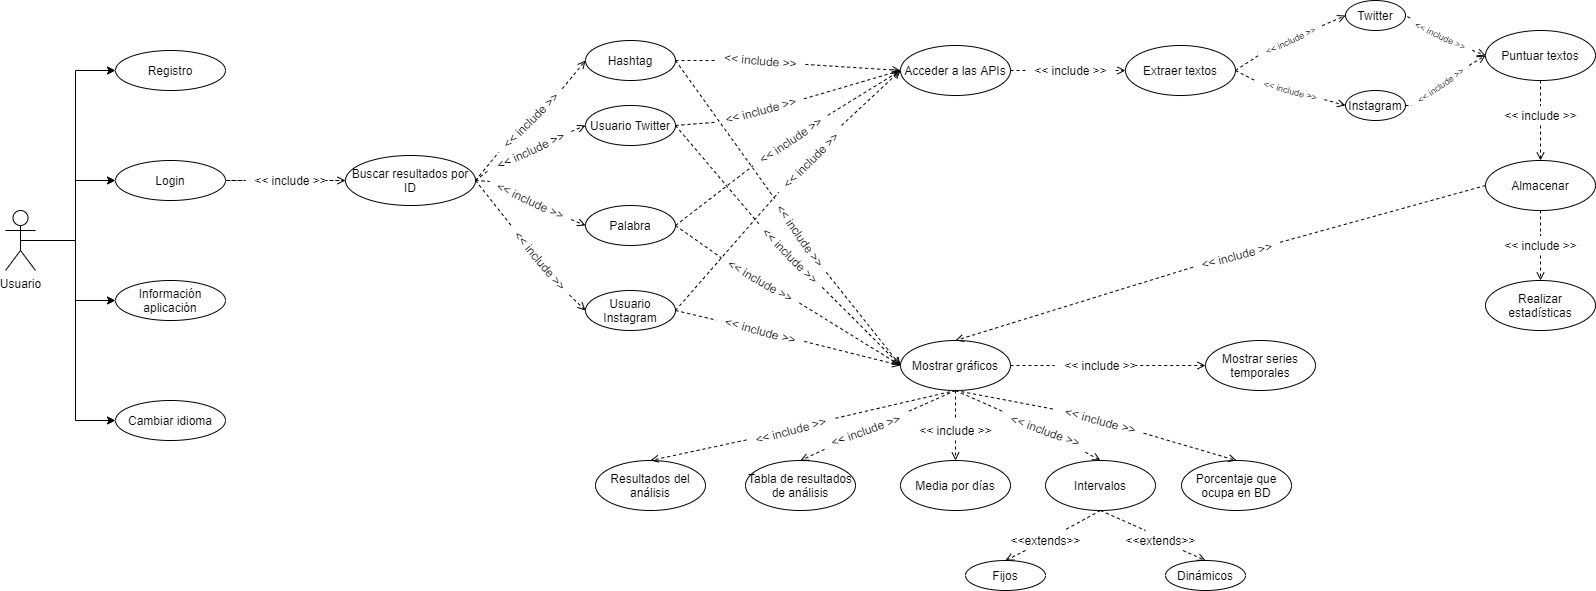
\includegraphics[scale=0.45]{img/CUSentinel.jpg}
    \caption{Diagrama de casos de uso}
\end{figure}
\end{landscape}




